
\subsection{Descrição do bloco operativo}

O bloco operativo é dividido basicamente em 3 loops, onde o primeiro loop vai
acumular os valores e o segundo loop tem o objetivo de estabilizar o calculo da
raiz quadrada. Quando este processo fica pronto o valor é comparado e
armazenado em um registrador. O terceiro loop serve para carregar o próximo
exemplo armazenado na memória e termina quando não existem mais exemplos para
serem comparados.

Para implementar este processo foram usados uma memória, um subtrator, um 
multiplicador, dois somadores, um acumulador, um bloco que calcula a raiz 
quadrada e um registrador.
Na implementação das operações e da memória foram utilizadas as 
\textit{megafunctions} para ponto flutuante do Quartus II.

\begin{figure}[h]
\centering
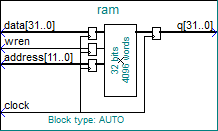
\includegraphics[width=.3\textwidth]{../apresentacao/ram}
\caption{\textit{Megafunction} ``RAM: 1-PORT''}
\label{fig:ram}
\end{figure}

A figura~\ref{fig:ram} descreve uma memória criada pelo 
\textit{MegaWizard Plug-In Manager} do Quartus II. 

O modelo utilizado no trabalho tem as seguintes entradas:
\begin{itemize}
\item \textit{data}~(32 bits): armazena o dado;
\item \textit{wren}~(1 bit): controla a escrita da memória;
\item \textit{address}~(11 bits): endereço de onde vai ser armazenado o dado;
\item \textit{clock}~(1 bit): relógio para sincronizar.
\end{itemize}

Este modelo de memória tem apenas uma saída de dados (q), que tem 32 bits e seu
valor depende da entrada \textit{address}. A memória é inicializada com
exemplos pelo componente \textit{altsyncram} atribuindo a entrada
\verb|init_file| um arquivo ``.mif''.

\begin{figure}[h]
\centering

\subfigure[ALTFP\_ADD\_SUB]{
	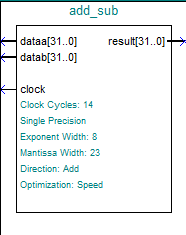
\includegraphics[width=.3\textwidth]{../apresentacao/add_sub}
	\label{fig:add_sub}
}
\quad
\subfigure[ALTFP\_MULT]{
	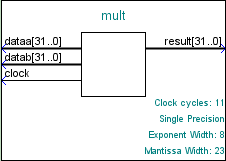
\includegraphics[width=.3\textwidth]{../apresentacao/mult}
	\label{fig:mult}
}
% Você pode adicionar mais subfigures aqui!
\label{fig:addsubmult}
\caption{\textit{Megafunctions} de soma/subtração e multiplicação}
\end{figure}

A figura~\ref{fig:add_sub} descreve a \textit{megafunction} de soma e subtração de
ponto flutuante do Quartus II. Ela foi configurada com formato de precisão
simples de ponto flutuante. Foi utilizado uma latência de 14 ciclos de relógio.

Para fazer a exponenciação foi utilizado um multiplicador de ponto flutuante a
partir da \textit{megafunction} \verb|ALTFP_MULT|. 
A figura~\ref{fig:mult} descreve a \textit{megafunction} de multiplicação de
ponto flutuante do Quartus II. Ela foi configurada com formato de precisão
simples de ponto flutuante. Foi utilizado uma latência de 11 ciclos de relógio.


As \textit{megafunctions} da figura~\ref{fig:addsubmult} foram utilizadas na 
implementação e tem as seguintes entradas:
\begin{itemize}
\item \textit{dataa} e \textit{datab}~(32 bits): dados a serem operados;
\item \textit{clock}~(1 bit): relógio para sincronizar.
\end{itemize}

Esta \textit{megafunction} tem apenas uma saída de resultado (\textit{result})
que tem 32 bits.

\begin{figure}[h]
\centering
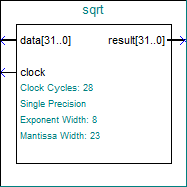
\includegraphics[width=.3\textwidth]{../apresentacao/sqrt}
\caption{\textit{Megafunction} ALTFP\_SQRT}
\label{fig:sqrt}
\end{figure}

A figura~\ref{fig:sqrt} descreve a \textit{megafunction} de raiz quadrada de
ponto flutuante do Quartus II. Ela foi configurada com formato de precisão
simples de ponto flutuante. Foi utilizado uma latência de 28 ciclos de relógio.

A \textit{megafunction} \verb|ALTFP_SQRT| utilizada no trabalho tem as
seguintes entradas:
\begin{itemize}
\item \textit{data}~(32 bits): dado a serem operados;
\item \textit{clock}~(1 bit): relógio para sincronizar.
\end{itemize}

Esta \textit{megafunction} tem apenas uma saída de resultado (\textit{result})
que tem 32 bits.


A figura~\ref{fig:compare} descreve a \textit{megafunction} de comparação de
ponto flutuante do Quartus II. Ela foi configurada com formato de precisão
simples de ponto flutuante. Foi utilizado uma latência de 3 ciclos de relógio.

\begin{figure}[h]
\centering
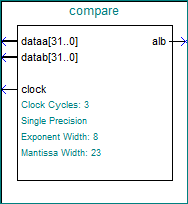
\includegraphics[width=.3\textwidth]{../apresentacao/compare}
\caption{\textit{Megafunction} ALTFP\_COMPARE}
\label{fig:compare}
\end{figure}

A \textit{megafunction} \verb|ALTFP_COMPARE| utilizada no trabalho tem as
seguintes entradas:
\begin{itemize}
\item \textit{dataa} e \textit{datab}~(32 bits): dados a serem operados;
\item \textit{clock}~(1 bit): relógio para sincronizar.
\end{itemize}

Esta \textit{megafunction} tem apenas uma saída que retorna um se a entrada
\textit{dataa} é menor do que a \textit{datab} caso contrario retorna zero.

\begin{figure}[h]
\centering
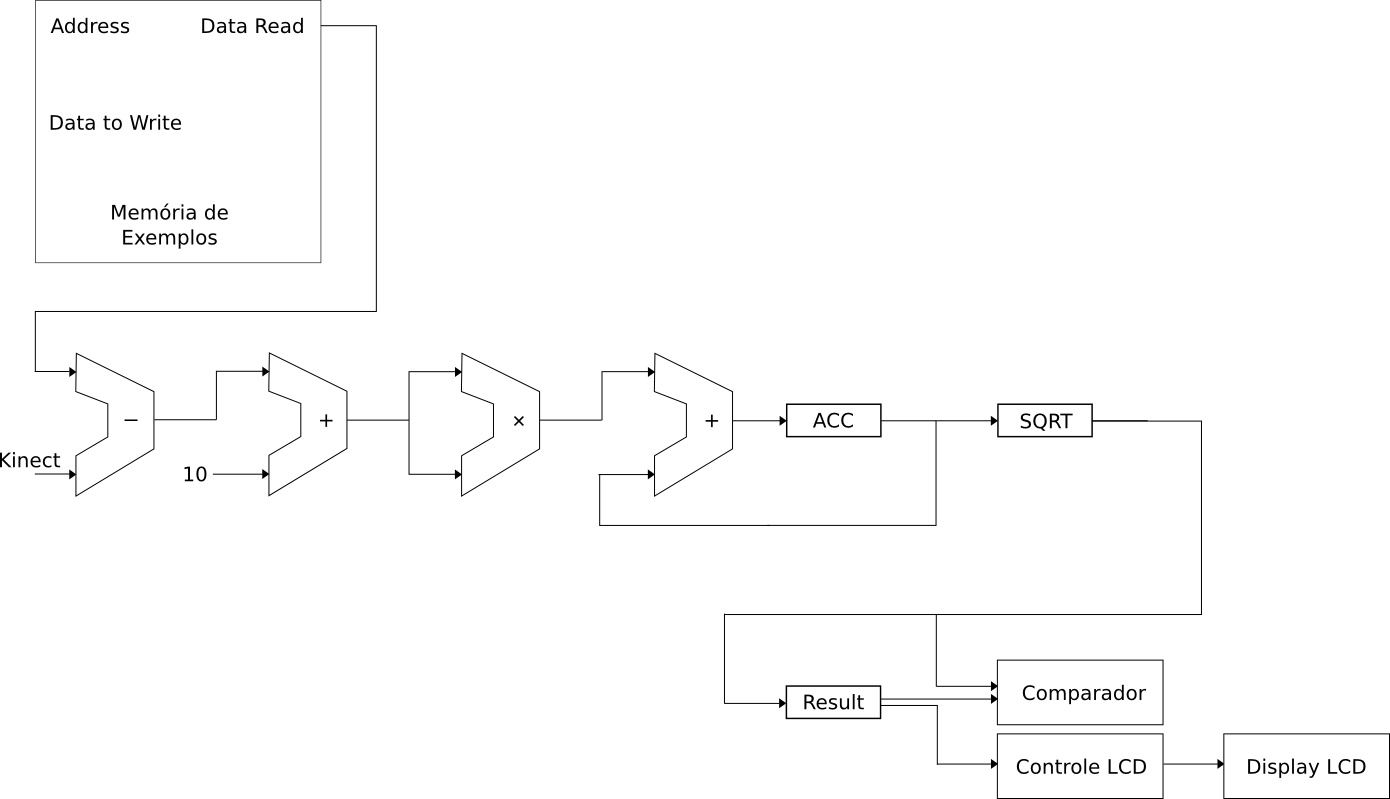
\includegraphics[width=.7\textwidth]{../apresentacao/knn_sem_controle}
\caption{Bloco operativo}
\label{fig:blocoperativo}
\end{figure}

A figura~\ref{fig:blocoperativo} apresenta o bloco operativo. O caminho de
dados inicia quando o bloco de aquisição de dados envia um sinal de que o 
\textit{array} com o frame do Kinect já esta preenchido.
